\documentclass{beamer}
\usepackage[utf8]{inputenc}

\usetheme{Madrid}
\usecolortheme{default}
\usepackage{amsmath,amssymb,amsfonts,amsthm}
\usepackage{txfonts}
\usepackage{tkz-euclide}
\usepackage{listings}
\usepackage{adjustbox}
\usepackage{array}
\usepackage{tabularx}
\usepackage{gvv}
\usepackage{lmodern}
\usepackage{circuitikz}
\usepackage{tikz}
\usepackage{graphicx}

\setbeamertemplate{page number in head/foot}[totalframenumber]

\usepackage{tcolorbox}
\tcbuselibrary{minted,breakable,xparse,skins}



\definecolor{bg}{gray}{0.95}
\DeclareTCBListing{mintedbox}{O{}m!O{}}{%
  breakable=true,
  listing engine=minted,
  listing only,
  minted language=#2,
  minted style=default,
  minted options={%
    linenos,
    gobble=0,
    breaklines=true,
    breakafter=,,
    fontsize=\small,
    numbersep=8pt,
    #1},
  boxsep=0pt,
  left skip=0pt,
  right skip=0pt,
  left=25pt,
  right=0pt,
  top=3pt,
  bottom=3pt,
  arc=5pt,
  leftrule=0pt,
  rightrule=0pt,
  bottomrule=2pt,
  toprule=2pt,
  colback=bg,
  colframe=orange!70,
  enhanced,
  overlay={%
    \begin{tcbclipinterior}
    \fill[orange!20!white] (frame.south west) rectangle ([xshift=20pt]frame.north west);
    \end{tcbclipinterior}},
  #3,
}
\lstset{
    language=C,
    basicstyle=\ttfamily\small,
    keywordstyle=\color{blue},
    stringstyle=\color{orange},
    commentstyle=\color{green!60!black},
    numbers=left,
    numberstyle=\tiny\color{gray},
    breaklines=true,
    showstringspaces=false,
}
\begin{document}

\title 
{4.3.22}
\date{August 31,2025}


\author 
{Kavin B-EE25BTECH11033}






\frame{\titlepage}
\begin{frame}{Question}
Find the ratio in which the line segment joining $\vec{A}(1,-5)$  and  $\vec{B}(-4,5)$ is divided by the $X$ axis. Also find the coordinates of the point of division.\\
\end{frame}



\begin{frame}{Theoretical Solution}

Let the vector $\vec{P}$ be the point on x-axis
\begin{align}
    \vec{P}=\begin{myvec}{x\\0}\end{myvec} \;, 
\end{align}
Given the points,
\begin{align}
    \vec{A}=\begin{myvec}{1\\-5}\end{myvec}\ \ \ 
    \vec{B}=\begin{myvec}{-4\\5}\end{myvec}
\end{align}
\bigskip
The points $\vec{A}$, $\vec{P}$, $\vec{B}$ are collinear.\\

\end{frame}

\begin{frame}{Formulae}
\textbf{Points $\vec{A}, \vec{P}, \vec{B}$ are defined to be collinear if}
\begin{align}
		\label{eq:line-rank-2}
		\rank{\myvec{\vec{P}-\vec{A}& \vec{B}-\vec{A}}} = 1
\end{align}
\begin{align}
            \vec{P}-\vec{A} = \myvec{x-1\\5}\\
            \vec{B}-\vec{A} = \myvec{-5\\10}
\end{align}    
\begin{align}
            \myvec{\vec{P}-\vec{A}& \vec{B}-\vec{A}} = \myvec{x-1 & -5\\5 & 10}
		\end{align}
\end{frame}

\begin{frame}{Theoretical Solution}

\begin{align}
R_1 \leftrightarrow R_2 \implies \myvec{5 & 10\\x-1 & -5}
\end{align}
\begin{align}
R_2 \rightarrow 2R_2 + R_1 \implies \myvec{5 & 10\\2x+3 & 0}
\end{align}
\begin{align}
R_2 \rightarrow R_2-(2x+3)R_1 \implies \myvec{1 & 2 \\ 0 & -4x-6}
\end{align}
For rank $1$, the second row must be zero:
\begin{align}
    -4x-6=0 \implies x=-3/2
\end{align}
\begin{center}
$\therefore \vec{P}=\begin{myvec}{-3/2\\0}\end{myvec}$
\end{center}
\end{frame}

\begin{frame}{Equation}
\textbf{Section formula for a vector $\vec{P}$ which divides the line formed by vectors $\vec{A}$ and $\vec{B}$ in the ratio k:1 is given by}
\begin{align}
    \vec{P}=\frac{k\vec{B}+\vec{A}}{k+1}
\end{align}
\begin{align}
			k\brak{\vec{P}-\vec{B}}&= \vec{A}-\vec{P}
\end{align}
\begin{align}
			\implies k &=
			\frac{\brak{\vec{A}-\vec{P}}^{\top}\brak{\vec{P}-\vec{B}}}{\norm{\vec{P}-\vec{B}}^2}
			\label{eq:section_formula-k}
\end{align}
\end{frame}
\begin{frame}{Theoretical Solution}
\begin{align}
\brak{\vec{A}-\vec{P}}^{\top}\brak{\vec{P}-\vec{B}} = \myvec{5/2 & -5}\myvec{5/2\\-5} = 125/4\\
{\norm{\vec{P}-\vec{B}}^2} = \brak{\sqrt{\brak{5/2}^2 + \brak{-5}^2}}^2 = 125/4
\end{align}

\begin{align}
\implies k &= 1
\end{align}

Therefore the ratio in which $\vec{P}$ divides the line segment joining the points $\vec{A}$ and $\vec{B}$ is $1:1$\\
\end{frame}

\begin{frame}{Plot}
    \centering
    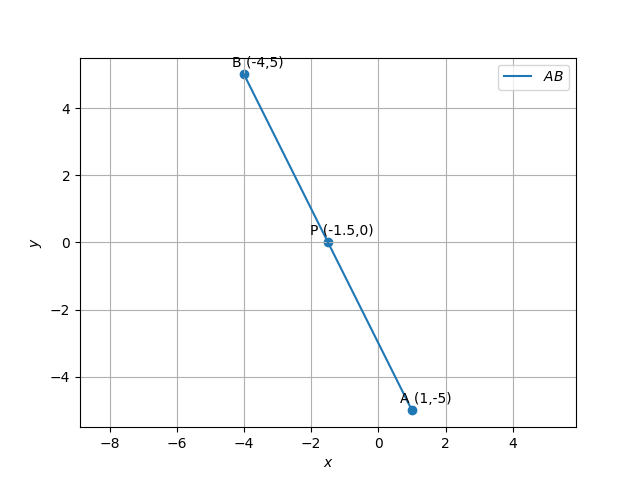
\includegraphics[width=\columnwidth, height=0.8\textheight, keepaspectratio]{figs/fig.png}     
\end{frame}


\end{document}
